
\documentclass[conference]{IEEEtran}
\usepackage{algorithm}
\usepackage{algpseudocode}
\usepackage{listings}
\usepackage{xcolor}
\usepackage{amsmath}
\usepackage{graphicx}
\usepackage{float}
\usepackage{booktabs}
\usepackage{url}
\usepackage{circuitikz}
\usepackage{booktabs}
\usepackage{array}
\usepackage{subcaption}
%\usepackage{gvv}
\usepackage{gvv-book}


% Define custom colors
\definecolor{codegreen}{rgb}{0,0.6,0}
\definecolor{codegray}{rgb}{0.5,0.5,0.5}
\definecolor{codepurple}{rgb}{0.58,0,0.82}
\definecolor{backcolour}{rgb}{0.95,0.95,0.92}

% Setup the listings package for C++
\lstset{
    language=C++,
    backgroundcolor=\color{backcolour},   
    commentstyle=\color{codegreen},
    keywordstyle=\color{blue},
    numberstyle=\tiny\color{codegray},
    stringstyle=\color{codepurple},
    basicstyle=\ttfamily\footnotesize,
    breakatwhitespace=false,         
    breaklines=true,                 
    captionpos=b,                    
    keepspaces=true,                 
    numbers=left,                    
    numbersep=5pt,                  
    showspaces=false,                
    showstringspaces=false,
    showtabs=false,                  
    tabsize=2
}
\title{Implementation of Indoor Positioning System using Ultra Wide Bandwidth(UWB)}

\author{
\IEEEauthorblockN{Indhiresh S, Kavin B}
\IEEEauthorblockA{
Department of Electrical Engineering\\
IIT Hyderabad\\
Email: ee25btech11027@iith.ac.in, ee25btech11033@iith.ac.in}
}

\begin{document}

\maketitle
\begin{abstract}
This documentation presents the development of a real-time, high-precision indoor positioning system utilizing Ultra-Wideband (UWB) technology. Because traditional global positioning systems fail to provide reliable coverage in indoor environments, this project leverages the ultra-wide frequency spectrum and short pulse duration of UWB RF signals to achieve centimeter-level spatial localization. By utilizing Time-of-Flight (ToF) ranging techniques, precise distances are calculated between a mobile UWB tag and a network of stationary anchors. These ranges are then processed through a 2D trilateration algorithm to dynamically compute the mobile tag's exact X and Y spatial coordinates. The localization data is edge-computed by an integrated microcontroller, which concurrently operates as a web server to host a live HTML5 canvas interface, allowing for the real-time visualization of the tracking data. Ultimately, this system demonstrates a robust, low-latency, and highly accurate solution for continuous indoor tracking, inherently overcoming common indoor RF challenges such as multipath interference.
\end{abstract}

\begin{IEEEkeywords}
Ultra-Wideband (UWB), Indoor Positioning System (IPS), Time-of-Flight (ToF), Trilateration Algorithm, Real-Time Spatial Tracking, Edge Computing
\end{IEEEkeywords}

\section{Introduction}

\subsection{Background and Motivation}
The proliferation of location-based services has driven a massive demand for accurate spatial tracking. While the Global Positioning System (GPS) is highly effective for outdoor navigation, it is fundamentally flawed in indoor environments. Satellite signals suffer from severe attenuation when passing through building materials, and the presence of walls and furniture creates complex multipath propagation. Consequently, GPS and other traditional radio-frequency tracking methods often yield positional errors measured in meters, which is unacceptable for precise indoor applications such as autonomous navigation, asset tracking, and smart environment automation. This creates a critical need for an alternative localization technology designed specifically for the unique challenges of indoor spaces.

\subsection{Ultra-Wideband (UWB) Technology}
To bridge the gap in indoor localization, Ultra-Wideband (UWB) technology has emerged as a superior solution. Unlike traditional narrowband systems that rely on signal strength (RSSI) to estimate distance, UWB operates across a massive frequency spectrum (typically 500 MHz or more) using extremely short, nanosecond-scale radio pulses. This unique physical characteristic allows UWB receivers to accurately distinguish between the direct line-of-sight signal and delayed multipath reflections. By measuring the precise Time-of-Flight (ToF) of these pulses traveling at the speed of light, UWB systems can calculate physical distances with centimeter-level accuracy, making it an ideal foundation for high-precision tracking.

\subsection{Project Scope and Objectives}
This project details the design and implementation of a custom UWB-based Indoor Positioning System (IPS). The primary objective is to develop a reliable, edge-computed tracking solution capable of real-time spatial localization. The system architecture consists of a mobile UWB tag and a network of fixed UWB anchors. By continually polling the ToF between the tag and the anchors, the system generates high-fidelity distance measurements. These ranges are actively processed through a 2D trilateration algorithm on a central microcontroller to compute the exact Cartesian coordinates ($X$ and $Y$) of the target. Finally, to ensure accessibility and immediate visual feedback, the hardware concurrently operates as a local web server, broadcasting the computed coordinates to a live HTML5 graphical interface.

\section{Methodology}

\subsection{System Architecture}
The proposed Indoor Positioning System (IPS) is built upon a centralized edge-computing architecture. The physical setup consists of three stationary Ultra-Wideband (UWB) reference nodes, designated as anchors, and one mobile UWB node, designated as the tag. The tag continuously broadcasts ranging pulses to the anchors, which process the signals to determine precise radial distances. An integrated microcontroller (acting as the central processing unit) aggregates these raw distance metrics, applies software-level outlier rejection, and computes the final spatial coordinates.

\subsection{Time-of-Flight (ToF) Ranging}
UWB technology relies on the transmission of nanosecond-scale radio pulses. By measuring the exact time it takes for a pulse to travel from the tag to an anchor and back, the system calculates the physical distance $r$. This relationship is fundamentally defined by the equation:
\begin{equation}
    r = c \times \frac{t_{ToF}}{2} = c \times \frac{(T_{recv} - T_{sent}) - \text{Delay}}{2}
\end{equation}
where $c$ is the speed of light in a vacuum ($\approx 3 \times 10^8$ m/s), and $t_{ToF}$ is the total round-trip time.
\begin{figure}[H]
    \centering
    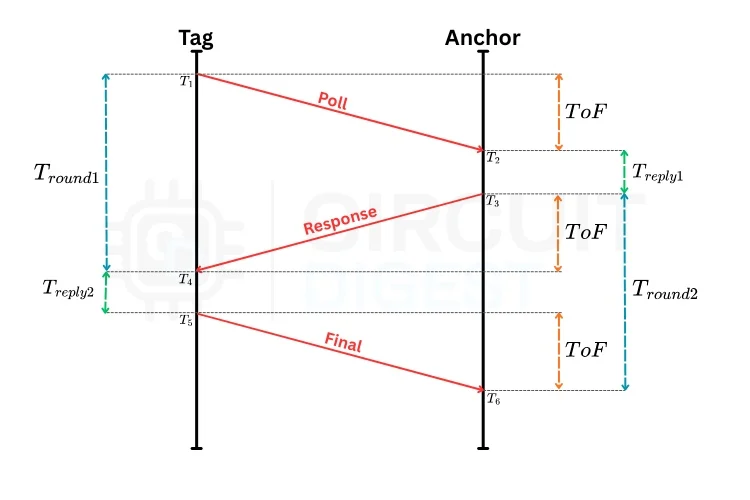
\includegraphics[width=0.5\textwidth]{figs/tof.png}
    \caption*{}
    \label{fig:tof}
\end{figure}

\subsection{2D Trilateration Algorithm}
Once the radial distances from the three anchors ($r_1, r_2, r_3$) are acquired, a 2D trilateration algorithm is employed to find the tag's exact spatial intersection. To optimize the computational load on the microcontroller, the coordinate system is aligned such that Anchor 1 is at the origin $(0,0)$, Anchor 2 lies on the x-axis at $(d,0)$, and Anchor 3 is located at an arbitrary point $(i,j)$.

The system of geometric equations representing the three intersecting ranging circles is:
\begin{align}
    r_1^2 &= x^2 + y^2 \\
    r_2^2 &= (x - d)^2 + y^2 \\
    r_3^2 &= (x - i)^2 + (y - j)^2
\end{align}

By expanding and algebraically manipulating these equations, the exact $x$ and $y$ coordinates of the mobile tag can be computed dynamically. The microcontroller executes the following simplified formulas in real-time:
\begin{equation}
    x = \frac{r_1^2 - r_2^2 + d^2}{2d}
\end{equation}
\begin{equation}
    y = \frac{r_1^2 - r_3^2 + i^2 + j^2 - 2ix}{2j}
\end{equation}

This streamlined algebraic approach provides a highly deterministic and computationally efficient method for real-time edge processing without the need for complex matrix inversions.
\begin{figure}[H]
    \centering
    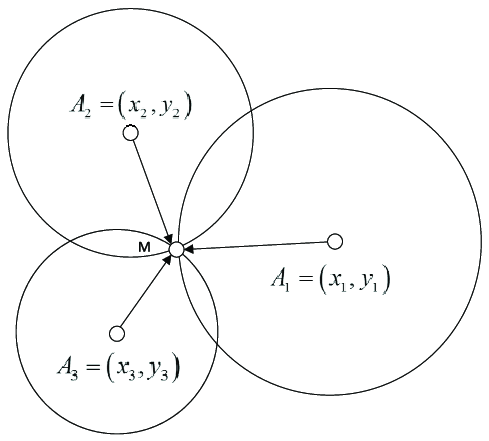
\includegraphics[width=0.4\textwidth]{figs/trilla.png}
    \caption*{}
    \label{fig:trilla}
\end{figure}

\section{IMPLEMENTATION USING SDR}
To gain full control over the physical layer, dedicated UWB modules were replaced with ADALM-Pluto Software Defined Radios (SDRs). The SDRs were unlocked via SSH to support frequencies up to 6 GHz , and all signal processing logic was transitioned to Python using \texttt{numpy} 

For Time-of-Flight ranging, the system utilizes a custom Zadoff-Chu pulse. The Tag transmits this sequence while initiating a timer, and the Anchor immediately reflects it back. Upon reception, the Tag performs a digital cross-correlation against the known sequence to pinpoint the exact peak arrival time, thereby determining the signal's round-trip time.

\subsection{Critical Challenges and Observations}

Transitioning from hardware-timed UWB modules to Software Defined Radios introduced several severe bottlenecks and processing latency issues:

\begin{itemize}
    \item \textbf{USB Power Bottleneck:} Two ADALM-Pluto SDRs draw approximately 1A of combined current, which caused standard laptop ports to brown out and repeatedly crash the network. This was resolved by connecting the devices to entirely separate USB buses on different sides of the host machine.
    \item \textbf{Network Routing Conflicts:} The Ubuntu host OS struggled to route traffic simultaneously to two different subnets (2.x and 3.x) on a single interface. Manual IP aliasing using the \texttt{sudo ip addr add} command was required to force the connections.
    \item \textbf{The "100 km" Offset Error:} Initial testing consistently reported massive distance measurements between 100 km and 200 km, despite the SDRs being placed exactly 1 meter apart. This fundamental error was primarily driven by system latency. USB data transfers and Python processing added an approximate 0.33 ms delay. Because radio waves travel at $300 \text{ km/ms}$, this microsecond delay translated mathematically into a $\approx 100 \text{ km}$ physical offset.
    \item \textbf{False Noise Detection and CFO:} Without a defined correlation threshold, the receiver triggered on random RF noise spikes instead of the true signal, returning erratic distances. Furthermore, unsynchronized clocks between the Tag and Anchor caused Carrier Frequency Offset (CFO), which smeared the Zadoff-Chu sequence's correlation peak and caused the algorithm to miss the true arrival time.
    \item \textbf{Processing Jitter:} Because standard Linux distributions are not Real-Time Operating Systems (RTOS), background tasks and OS scheduling paused the Python script randomly. Coupled with USB 2.0 polling latency ($\pm 125 \mu s$), the processing time was highly variable. A timing jitter of just $1 \mu s$ creates a 300-meter distance error, demonstrating the extreme instability of software-reliant Time-of-Flight ranging.
\end{itemize}

\subsection{Results}
In conclusion, replacing dedicated hardware with Software Defined Radios (SDRs) like the ADALM-Pluto fundamentally fails for Time-of-Flight (ToF) ranging due to insurmountable system latencies. Because electromagnetic waves travel at light speed, the inherent 0.33 ms delay from USB transfers and Python processing mathematically fabricates massive distance errors of roughly 100 kilometers. Furthermore, relying on a non-Real-Time Operating System (RTOS) introduces unpredictable processing jitter, while unsynchronized clocks cause Carrier Frequency Offsets (CFO) that smear the correlation peaks and trigger false noise detections. Ultimately, while SDRs offer excellent physical layer control, their tethered, software-reliant architecture is simply too unstable to support the microsecond-level precision required for functional UWB positioning.
\newpage
\section{IMPLEMENTATION USING ESP32: ANALYTICAL APPROACH}

\subsection{HARDWARE REQUIREMENTS}
\begin{itemize}
    \item \textbf{Tracking Tag:} ESP32 Microcontroller (FTM/802.11mc compatible, e.g., ESP32-S2 or ESP32-S3).
    \item \textbf{Anchors:} 3x Wi-Fi Access Points or ESP32 nodes configured as FTM responders.
    \item \textbf{Monitoring Device:} Smartphone or PC with Wi-Fi capabilities and a modern web browser.
\end{itemize}

\subsection{SYSTEM ARCHITECTURE}
The positioning system relies on calculating the distance between the mobile tag and three fixed anchors located at known coordinates: A1(0,0), A2(10,0), and A3(5,8).

\subsubsection{Time of Flight (ToF) Measurement}
The ESP32 initiates an FTM burst (typically 32 packets) to each anchor. By measuring the Round Trip Time (RTT) of these radio frequency bursts, the distance is mathematically derived using the speed of light.

\subsubsection{Asynchronous Web Server}
To prevent blocking operations during FTM packet collection, the ESP32 hosts a local SoftAP network (\texttt{ESP32-Live-Map}). A lightweight web server handles incoming client requests and serves a dynamic HTML5 UI that fetches JSON coordinate data.

\subsection{FILTERING AND GEOMETRIC TRILATERATION}

\subsubsection{Moving Median Filter}
To isolate the true line-of-sight distance from anomalous readings, a 5-point rolling window is utilized. The array is sorted using a bubble sort algorithm, and the exact median value is extracted to strip sudden multipath spikes.

\subsubsection{2D Trilateration Math}
The intersecting X and Y coordinates of the tag are calculated using standard algebraic trilateration derivations based on the filtered radii:

$$x = \frac{r_1^2 - r_2^2 + d^2}{2d}$$
$$y = \frac{r_1^2 - r_3^2 + i^2 + j^2 - 2ix}{2j}$$

where $d$ is the x-coordinate of Anchor 2, and $(i, j)$ are the coordinates of Anchor 3.
\newpage
\subsection{CODE IMPLEMENTED}
\begin{lstlisting}[language=C++]
/* --- Analytical approach for UWB Positioning system  ---
   Anchors: A1(0,0), A2(10,0), A3(5,8)

*/

#include "WiFi.h"
#include <WebServer.h>
#include <math.h>

// ==========================================
// 1. CONFIGURATION
// ==========================================
float anchors[3][2] = {
  {0.00,  0.00},  // Anchor 01
  {10.00, 0.00},  // Anchor 02
  {5.00,  8.00}   // Anchor 03
};
String anchorNames[] = {"FTM_Anchor_01", "FTM_Anchor_02", "FTM_Anchor_03"};
float distance_offset = 0.0; 

// ==========================================
// 2. FILTERING & CACHED VARIABLES
// ==========================================
float dist_history[3][5]; 
int history_idx[3] = {0, 0, 0};
float smoothed_distances[3] = {0, 0, 0};
bool first_reading[3] = {true, true, true}; 

volatile bool got_data = false;
float last_raw_val = 0;

// Cached Wi-Fi Data (Prevents scanning in the loop)
uint8_t anchorBSSIDs[3][6];
int anchorChannels[3];
bool anchorFound[3] = {false, false, false};

// Coordinate Globals for Web UI
float posX = 0.0;
float posY = 0.0;

WebServer server(80);

// ==========================================
// 3. THE WEB UI (HTML + JAVASCRIPT)
// ==========================================
const char index_html[] PROGMEM = R"rawliteral(
<!DOCTYPE html>
<html>
<head>
  <meta name="viewport" content="width=device-width, initial-scale=1">
  <title>ESP32 Indoor GPS</title>
  <style>
    body { font-family: Arial; text-align: center; background-color: #222; color: #fff; margin: 0; padding: 20px;}
    canvas { background-color: #111; border: 2px solid #555; border-radius: 5px; box-shadow: 0px 0px 15px rgba(0,255,255,0.2); margin-top: 10px; max-width: 100%;}
    .stats { font-size: 1.2em; font-weight: bold; color: #00FFCC; margin-top: 15px; }
    .debug { font-size: 0.9em; color: #aaa; margin-top: 5px; }
  </style>
</head>
<body>
  <h2>Live Tracking (10m x 8m)</h2>
  
  <canvas id="mapCanvas" width="400" height="320"></canvas>
  
  <div class="stats" id="coords">X: 0.00 m | Y: 0.00 m</div>
  <div class="debug" id="dists">A1: 0m | A2: 0m | A3: 0m</div>

  <script>
    const canvas = document.getElementById('mapCanvas');
    const ctx = canvas.getContext('2d');
    const scale = 40; // 40 pixels = 1 meter
    
    function drawGrid() {
      ctx.clearRect(0, 0, canvas.width, canvas.height);
      
      // Draw Grid Lines
      ctx.strokeStyle = "#333";
      for(let i=0; i<10; i++) {
        ctx.beginPath(); ctx.moveTo(i*scale, 0); ctx.lineTo(i*scale, 320); ctx.stroke();
        ctx.beginPath(); ctx.moveTo(0, i*scale); ctx.lineTo(400, i*scale); ctx.stroke();
      }

      // Draw Anchors
      ctx.fillStyle = "#00FFCC";
      ctx.fillRect(0, 320 - 10, 10, 10); // A1 (0,0)
      ctx.fillRect(10 * scale - 10, 320 - 10, 10, 10); // A2 (10,0)
      ctx.fillRect(5 * scale - 5, 320 - (8 * scale), 10, 10); // A3 (5,8)
      
      ctx.fillStyle = "#fff";
      ctx.font = "12px Arial";
      ctx.fillText("A1(0,0)", 15, 310);
      ctx.fillText("A2(10,0)", 340, 310);
      ctx.fillText("A3(5,8)", 215, 20);
    }

    function updateMap() {
      fetch('/data')
        .then(response => response.json())
        .then(data => {
          drawGrid();
          
          // Draw Tag
          let cx = data.x * scale;
          let cy = 320 - (data.y * scale); // Invert Y for canvas
          
          // Constrain dot to canvas bounds visually
          if(cx < 0) cx = 5; if(cx > 400) cx = 395;
          if(cy < 0) cy = 5; if(cy > 320) cy = 315;

          ctx.beginPath();
          ctx.arc(cx, cy, 8, 0, 2 * Math.PI);
          ctx.fillStyle = "#FF3366";
          ctx.fill();
          ctx.strokeStyle = "#fff";
          ctx.stroke();
          
          document.getElementById('coords').innerText = "X: " + data.x.toFixed(2) + " m | Y: " + data.y.toFixed(2) + " m";
          document.getElementById('dists').innerText = "A1: " + data.r1.toFixed(1) + "m | A2: " + data.r2.toFixed(1) + "m | A3: " + data.r3.toFixed(1) + "m";
        })
        .catch(err => console.log(err));
    }

    drawGrid();
    setInterval(updateMap, 400); // Fetch data every 0.4s
  </script>
</body>
</html>
)rawliteral";

// ==========================================
// 4. FTM EVENT HANDLER
// ==========================================
void onFtmReport(arduino_event_t *event) {
  wifi_event_ftm_report_t *report = &event->event_info.wifi_ftm_report;
  if (report->status == FTM_STATUS_SUCCESS) {
    last_raw_val = (report->dist_est / 100.0) + distance_offset;
    got_data = true;
  }
}

// ==========================================
// 5. SETUP
// ==========================================
void setup() {
  Serial.begin(115200);
  
  // Wi-Fi Setup: AP mode for Web Server, STA mode for FTM
  WiFi.mode(WIFI_AP_STA); 
  WiFi.softAP("ESP32-Live-Map", "12345678"); // Hotspot Name & Password
  WiFi.onEvent(onFtmReport, ARDUINO_EVENT_WIFI_FTM_REPORT);
  WiFi.setSleep(false);
  
  // Web Server Endpoints
  server.on("/", []() { 
    server.send(200, "text/html", index_html); 
  });
  
  server.on("/data", []() { 
    char json[100];
    sprintf(json, "{\"x\":%.2f, \"y\":%.2f, \"r1\":%.2f, \"r2\":%.2f, \"r3\":%.2f}", 
            posX, posY, smoothed_distances[0], smoothed_distances[1], smoothed_distances[2]);
    server.send(200, "application/json", json);
  });
  
  server.begin();
  
  Serial.println("\n--- 10m Stabilized System Starting ---");
  Serial.println("Scanning for Anchors...");

  // ONE-TIME SCAN FOR ANCHORS
  int n = WiFi.scanNetworks(false, false, false, 150); 
  for (int i = 0; i < n; i++) {
    for (int j = 0; j < 3; j++) {
      if (WiFi.SSID(i) == anchorNames[j]) {
        anchorChannels[j] = WiFi.channel(i);
        memcpy(anchorBSSIDs[j], WiFi.BSSID(i), 6);
        anchorFound[j] = true;
        Serial.printf("Found %s on Channel %d\n", anchorNames[j].c_str(), anchorChannels[j]);
      }
    }
  }
  WiFi.scanDelete(); // Free memory

  Serial.println("Connect Phone to Wi-Fi: ESP32-Live-Map");
  Serial.println("Open Browser to: http://192.168.4.1");
}

// ==========================================
// 6. MAIN LOOP
// ==========================================
void loop() {
  server.handleClient(); // Keep the website alive

  for (int j = 0; j < 3; j++) {
    if (anchorFound[j]) {
      got_data = false;
      
      // Request FTM using CACHED BSSID and Channel
      if (WiFi.initiateFTM(32, 0, anchorChannels[j], anchorBSSIDs[j])) {
         unsigned long start = millis();
         
         // Wait for data, feeding the web server
         while(!got_data && millis() - start < 1000) { 
           delay(10); 
           server.handleClient(); 
         }
         
         if(got_data && last_raw_val > 0.1 && last_raw_val < 30.0) {
           
           // Fill array on first reading to prevent ramp-up lag
           if (first_reading[j]) {
             for (int k = 0; k < 5; k++) dist_history[j][k] = last_raw_val;
             first_reading[j] = false;
           } else {
             dist_history[j][history_idx[j]] = last_raw_val;
             history_idx[j] = (history_idx[j] + 1) % 5;
           }
           
           // --- MEDIAN FILTER LOGIC ---
           float temp[5];
           
           // 1. Copy the history array
           for(int k=0; k<5; k++) {
             temp[k] = dist_history[j][k];
           }
           
           // 2. Bubble Sort the temporary array
           for(int p=0; p<4; p++) {
             for(int q=0; q<4-p; q++) {
               if(temp[q] > temp[q+1]) {
                 float t = temp[q];
                 temp[q] = temp[q+1];
                 temp[q+1] = t;
               }
             }
           }
           
           // 3. Extract the median value (middle element)
           smoothed_distances[j] = temp[2]; 
           // ---------------------------
         }
      }
      
      // Brief delay, feeding server
      unsigned long d_start = millis();
      while(millis() - d_start < 50) { server.handleClient(); delay(1); }
    }
  }

  // Only calculate XY if we have valid readings for all 3 anchors
  if (!first_reading[0] && !first_reading[1] && !first_reading[2]) {
    calculateXY();
  }
}

// ==========================================
// 7. TRILATERATION MATH
// ==========================================
void calculateXY() {
  float r1 = smoothed_distances[0];
  float r2 = smoothed_distances[1];
  float r3 = smoothed_distances[2];
  
  float d = anchors[1][0]; // 10.0
  float i = anchors[2][0]; // 5.0
  float j = anchors[2][1]; // 8.0

  float x = (pow(r1, 2) - pow(r2, 2) + pow(d, 2)) / (2 * d);
  float y = (pow(r1, 2) - pow(r3, 2) + pow(i, 2) + pow(j, 2) - (2 * i * x)) / (2 * j);

  if (isnan(x) || isnan(y)) return;

  // Update globals for the Web UI
  posX = x;
  posY = y;

  Serial.printf("DIST -> A1:%.2fm A2:%.2fm A3:%.2fm | POS -> X:%.2fm, Y:%.2fm\n", r1, r2, r3, x, y);
}
\end{lstlisting}

\subsection{EXPERIMENTAL RESULTS AND LIMITATIONS}
While the software architecture successfully processes FTM data, empirical testing revealed severe hardware and environmental limitations that restrict the practical application of purely geometric trilateration for indoor positioning.

\subsubsection{Outdoor vs. Indoor Performance}
Field experiments were conducted in both clear outdoor environments and enclosed indoor spaces. 
\begin{itemize}
    \item \textbf{Outdoor Environment:} In open-air conditions with a clear Line-of-Sight (LOS) between the tag and anchors, the system demonstrated an average positioning error of 1 to 2 meters. This establishes the baseline capability of the ESP32's FTM implementation under optimal conditions.
    \item \textbf{Indoor Environment:} When the identical setup was transitioned indoors, the system exhibited significantly higher error rates, often reporting distances that were mathematically impossible given the physical dimensions of the room.
\end{itemize}

\subsubsection{Multipath Interference and Signal Reflection}

The primary cause of the severe indoor inaccuracy is multipath propagation. In an indoor environment, 2.4 GHz Wi-Fi signals reflect heavily off walls, floors, ceilings, and metallic objects. Consequently, the ESP32 often receives delayed, reflected signals rather than the direct LOS signal. Because FTM relies strictly on the Time-of-Flight, these delayed reflections artificially inflate the calculated distance, completely corrupting the trilateration geometry. 

\subsubsection{Impossibility of Centimeter-Level Accuracy}
It must be explicitly stated that achieving centimeter-level accuracy using the ESP32 is a physical and mathematical impossibility. The resolution of FTM is directly constrained by the bandwidth of the Wi-Fi signal. Standard ESP32 hardware operates on a 20 MHz channel bandwidth, which limits the theoretical best-case distance resolution to the meter level. Unlike true Ultra-Wideband (UWB) technologies, which use wide bandwidths (500 MHz or more) to achieve very sharp, centimeter-accurate pulses, the ESP32 is fundamentally hardware-locked to meter-level accuracy.
\newpage
% ---------------------------------------------------------
\section{IMPLEMENTATION USING ESP32: MACHINE LEARNING APPROACH}

\subsection{OVERCOMING GEOMETRIC LIMITATIONS}
Because pure mathematical trilateration fails in multipath-heavy indoor environments, the system architecture can be adapted to utilize data-driven Machine Learning (ML) techniques. By treating the hardware biases and RF reflections as learnable patterns rather than geometric absolute values, the ESP32's meter-level limitations can be heavily mitigated.

\subsection{Baseline ML: Linear Regression (Least Squares Calibration)}
Similar to calibrating analog hardware sensors to account for static environmental variables, a foundational linear regression model was deployed to correct antenna phase center shifts and hardware delays. 

Using the Least Squares method, the system was trained on a dataset of known physical coordinates to mathematically map the erroneous measured FTM distances to the true physical distances. The data collected for this training phase is detailed in Table \ref{tab:calibration_data}.

\begin{table}[htbp]
\centering
\caption{Raw FTM Distance Dataset for ML Calibration}
\label{tab:calibration_data}
\begin{tabular}{|c|c|c|c|c|c|}
\hline
\textbf{S.NO} & \textbf{X} & \textbf{Y} & \textbf{Dist\_A1} & \textbf{Dist\_A2} & \textbf{Dist\_A3} \\
\hline
1 & 0 & 0 & 0.1 & 15.9 & 22.4 \\
\hline
2 & 0 & 2 & 8.6 & 12.4 & 12.9 \\
\hline
3 & 0 & 4 & 11.8 & 13.3 & 18.1 \\
\hline
4 & 0 & 6 & 16.5 & 14.3 & 10.2 \\
\hline
5 & 0 & 8 & 9.3 & 14.4 & 7.5 \\
\hline
6 & 2 & 2 & 5.4 & 18.8 & 10.5 \\
\hline
7 & 2 & 4 & 4.7 & 10.8 & 14.4 \\
\hline
8 & 2 & 6 & 6.8 & 12.6 & 9.8 \\
\hline
9 & 4 & 2 & 16.1 & 11.6 & 16.9 \\
\hline
10 & 4 & 4 & 6.6 & 10.1 & 10.9 \\
\hline
11 & 4 & 6 & 7.8 & 15.6 & 15.3 \\
\hline
12 & 6 & 2 & 7.5 & 10.1 & 9.0 \\
\hline
13 & 6 & 4 & 7.3 & 7.7 & 8.6 \\
\hline
14 & 6 & 6 & 9.0 & 8.3 & 4.3 \\
\hline
15 & 8 & 2 & 9.2 & 4.3 & 9.8 \\
\hline
16 & 8 & 4 & 12.4 & 10.3 & 5.7 \\
\hline
17 & 8 & 6 & 10.8 & 12.2 & 6.9 \\
\hline
18 & 8 & 8 & 13.8 & 15.6 & 4.3 \\
\hline
19 & 10 & 0 & 14.3 & 1.1 & 17.3 \\
\hline
20 & 10 & 2 & 8.8 & 5.8 & 9.4 \\
\hline
21 & 10 & 4 & 14.7 & 6.5 & 8.0 \\
\hline
22 & 10 & 6 & 18.3 & 8.8 & 7.5 \\
\hline
23 & 10 & 8 & 15.2 & 12.2 & 7.0 \\
\hline
24 & 5 & 0 & 5.4 & 7.8 & 9.6 \\
\hline
25 & 5 & 8 & 16.5 & 16.2 & 1.2 \\
\hline
\end{tabular}
\end{table}

To derive the optimal calibration constants, the Ordinary Least Squares (OLS) method was formulated using matrix algebra. For each anchor located at $(X_A, Y_A)$, the true Euclidean distance vector $Y$ ($25 \times 1$) for the $n=25$ calibration points is computed as:
$$y_i = \sqrt{(X_i - X_A)^2 + (Y_i - Y_A)^2}$$

The measured FTM distances populate the design matrix $X$ ($25 \times 2$), where the first column consists of ones to account for the intercept $c$, and the second column contains the raw distance readings $d_{measured}$:
$$\vec{X} = \begin{bmatrix} 1 & x_1 \\ 1 & x_2 \\ \vdots & \vdots \\ 1 & x_{25} \end{bmatrix}, \quad \vec{Y}= \begin{bmatrix} y_1 \\ y_2 \\ \vdots \\ y_{25} \end{bmatrix}, \quad \vec{\beta} = \begin{bmatrix} c \\ m \end{bmatrix}$$

The coefficient vector $\vec{\beta}$ is solved by minimizing the residual sum of squares using the closed-form normal equation:
$$\vec{\beta}= (\vec{X}^T \vec{X})^{-1} \vec{X}^T \vec{Y}$$

By applying this matrix transformation to the dataset in Table \ref{tab:calibration_data} for each respective anchor---$A_1(0,0)$, $A_2(10,0)$, and $A_3(5,8)$---the derived regression constants optimized for the three ESP32 anchors are:
\begin{itemize}
    \item \textbf{Anchor 1:} $m = 0.4614, c = 2.5134$
    \item \textbf{Anchor 2:} $m = 0.6145, c = 0.3300$
    \item \textbf{Anchor 3:} $m = 0.2887, c = 2.4097$
\end{itemize}
By applying these trained weights ($d_{true} = m \cdot d_{measured} + c$) before executing the trilateration algorithm, the system effectively normalizes the non-linear hardware delays that the geometric approach ignores.

\subsection{System Visualizations and Images}

% The asterisk in figure* makes it span across both columns!
\begin{figure*}[htbp]
    \centering
    
    % --- ROW 1 ---
    \begin{subfigure}[b]{0.45\textwidth}
        \centering
        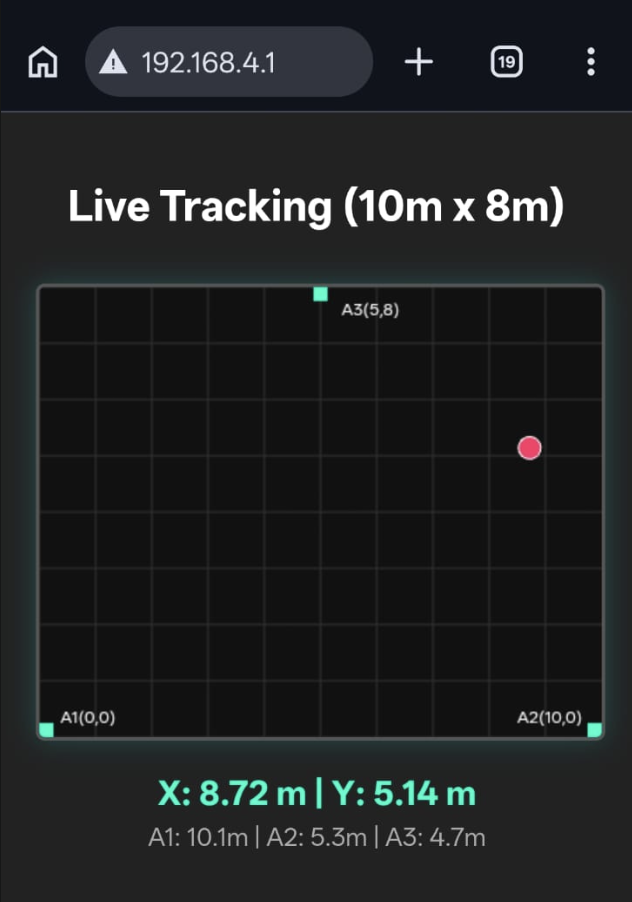
\includegraphics[width=\textwidth]{figs/picc1.png}
        \caption*{(8,6)}
        \label{fig:img1}
    \end{subfigure}
    \hfill
    \begin{subfigure}[b]{0.45\textwidth}
        \centering
        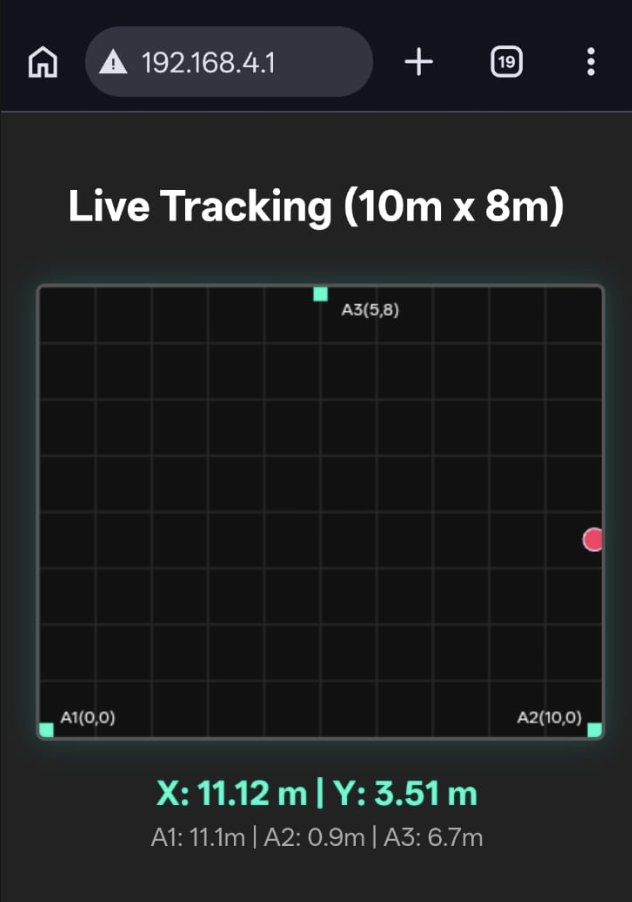
\includegraphics[width=\textwidth]{figs/picc2.png}
        \caption*{(10,0)}
        \label{fig:img2}
    \end{subfigure}
    
    \vspace{0.5cm} % Adds a little vertical space between rows
    
    % --- ROW 2 ---
    \begin{subfigure}[b]{0.45\textwidth}
        \centering
        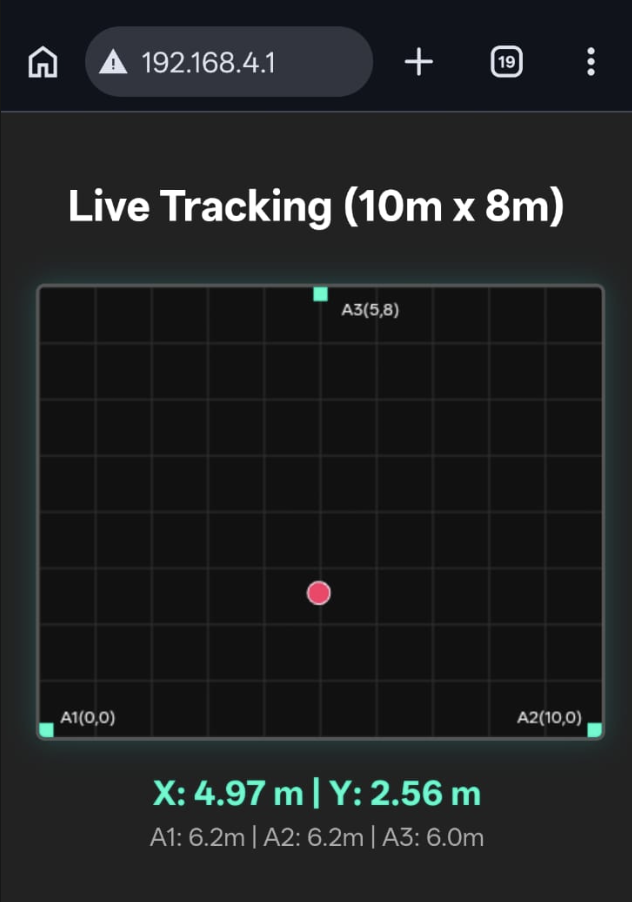
\includegraphics[width=\textwidth]{figs/picc3.png}
        \caption*{(4,4)}
        \label{fig:img3}
    \end{subfigure}
    \hfill
    \begin{subfigure}[b]{0.45\textwidth}
        \centering
        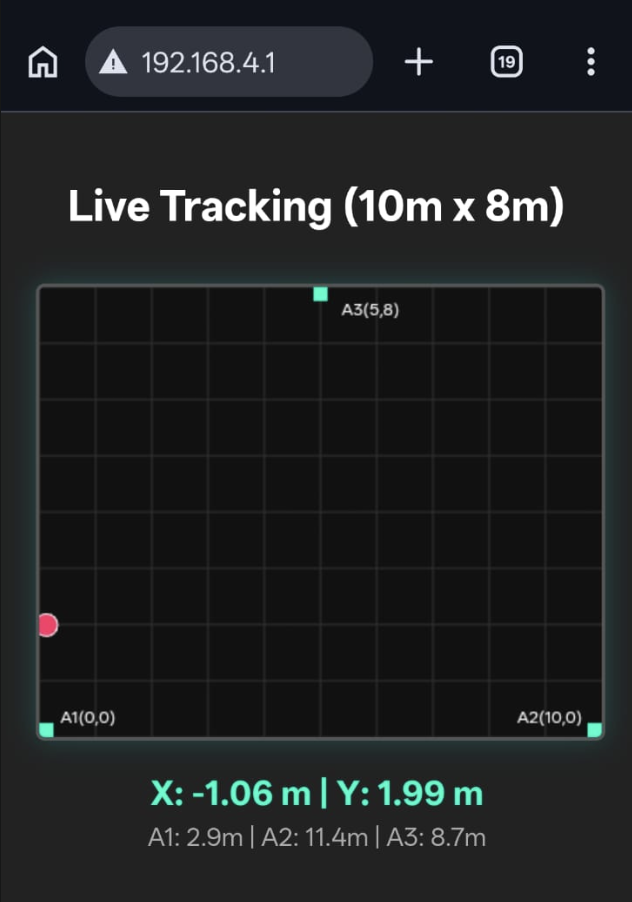
\includegraphics[width=\textwidth]{figs/picc4.png}
        \caption*{(0,0)}
        \label{fig:img4}
    \end{subfigure}
    
    \vspace{0.5cm}
\end{figure*}
\begin{figure*}[htbp]
    \centering
    % --- ROW 3 ---
    \begin{subfigure}[b]{0.45\textwidth}
        \centering
        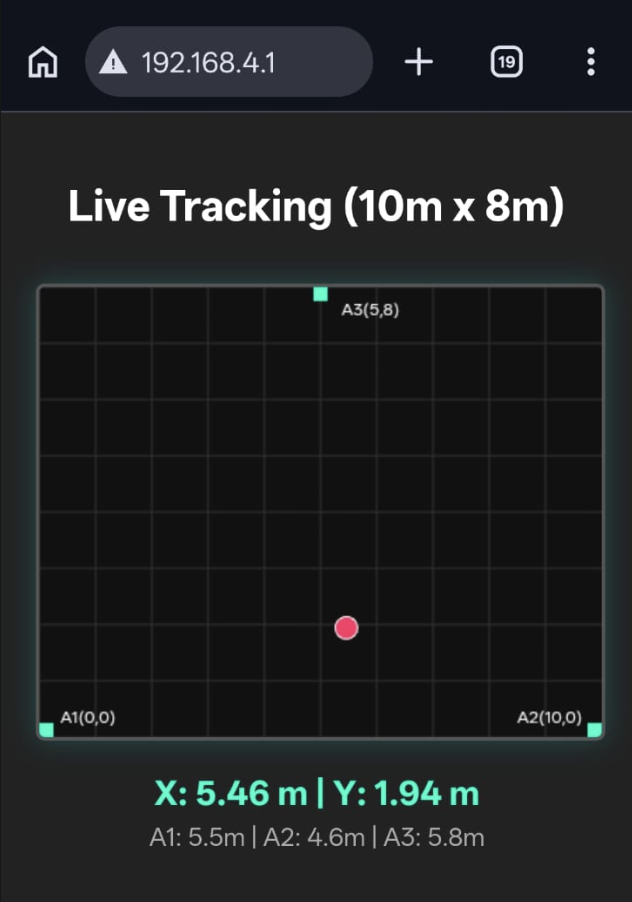
\includegraphics[width=\textwidth]{figs/picc5.png}
        \caption*{(6,2)}
        \label{fig:img5}
    \end{subfigure}
    \hfill
    \begin{subfigure}[b]{0.45\textwidth}
        \centering
        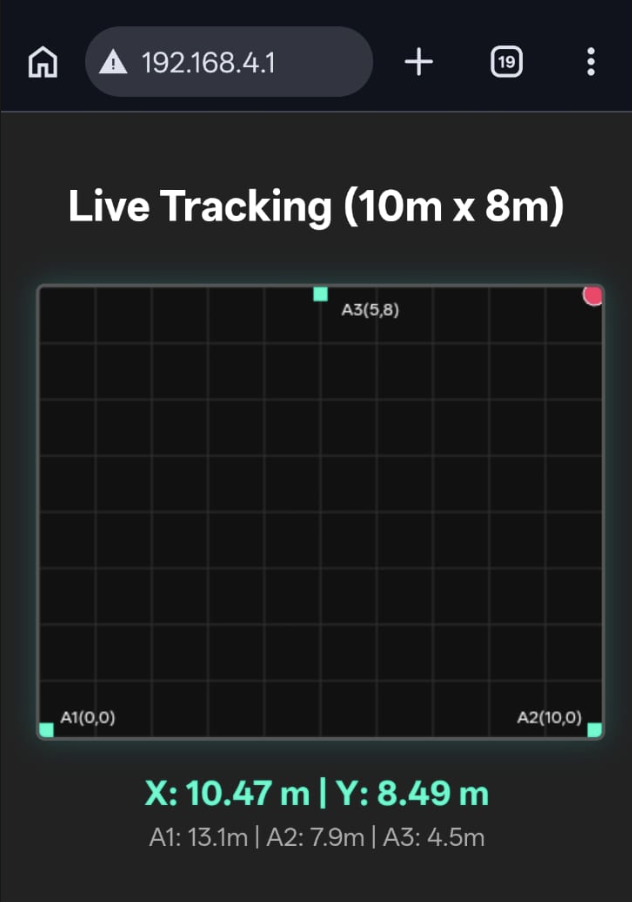
\includegraphics[width=\textwidth]{figs/picc6.png}
        \caption*{(8,6)}
        \label{fig:img6}
    \end{subfigure}

    \vspace{0.5cm}
    
    % --- ROW 4 ---
    \begin{subfigure}[b]{0.45\textwidth}
        \centering
        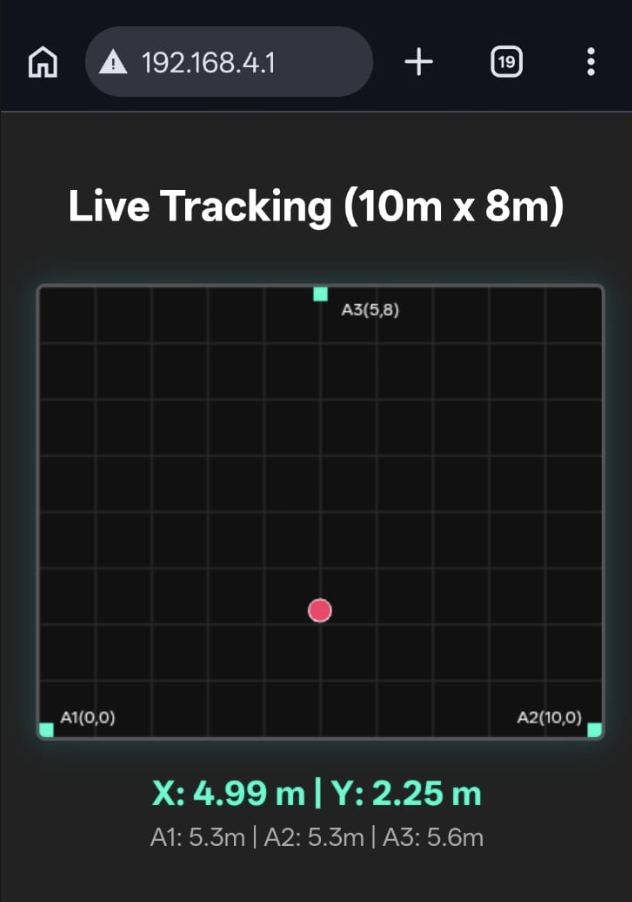
\includegraphics[width=\textwidth]{figs/picc7.png}
        \caption*{(4,2)}
        \label{fig:img7}
    \end{subfigure}
    \hfill
    \begin{subfigure}[b]{0.45\textwidth}
        \centering
        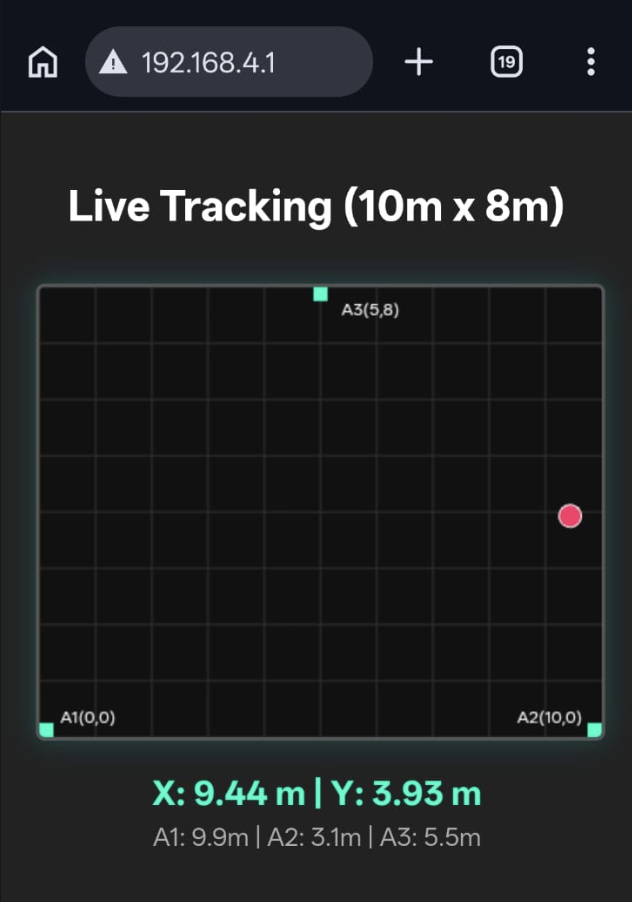
\includegraphics[width=\textwidth]{figs/picc8.png}
        \caption*{(8,2)}
        \label{fig:img8}
    \end{subfigure}
    \label{fig:all_8_images}
\end{figure*}
\newpage
\\
\subsection{Code Implemented}
\begin{lstlisting}[language=C++]
/* --- ML approach for UWB Positioning system ---
   Anchors: A1(0,0), A2(10,0), A3(5,8)
*/

#include "WiFi.h"
#include <WebServer.h>
#include <math.h>

// ==========================================
// 1. CONFIGURATION & CALIBRATION
// ==========================================
float anchors[3][2] = {
  {0.00,  0.00},  // Anchor 01
  {10.00, 0.00},  // Anchor 02
  {5.00,  8.00}   // Anchor 03
};
String anchorNames[] = {"FTM_Anchor_01", "FTM_Anchor_02", "FTM_Anchor_03"};

// LEAST SQUARES CALIBRATION CONSTANTS (Calculated from your 25-point dataset)
// Format: d_true = (m * d_measured) + c
float A1_m = 0.4614; float A1_c = 2.5134;
float A2_m = 0.6145; float A2_c = 0.3300;
float A3_m = 0.2887; float A3_c = 2.4097;

// ==========================================
// 2. FILTERING & CACHED VARIABLES
// ==========================================
float dist_history[3][5]; 
int history_idx[3] = {0, 0, 0};
float smoothed_distances[3] = {0, 0, 0};
float calibrated_distances[3] = {0, 0, 0}; 
bool first_reading[3] = {true, true, true}; 

volatile bool got_data = false;
float last_raw_val = 0;

uint8_t anchorBSSIDs[3][6];
int anchorChannels[3];
bool anchorFound[3] = {false, false, false};

float posX = 0.0;
float posY = 0.0;

WebServer server(80);

// ==========================================
// 3. THE WEB UI (HTML + JAVASCRIPT)
// ==========================================
const char index_html[] PROGMEM = R"rawliteral(
<!DOCTYPE html>
<html>
<head>
  <meta name="viewport" content="width=device-width, initial-scale=1">
  <title>ESP32 Indoor GPS</title>
  <style>
    body { font-family: Arial; text-align: center; background-color: #222; color: #fff; margin: 0; padding: 20px;}
    canvas { background-color: #111; border: 2px solid #555; border-radius: 5px; box-shadow: 0px 0px 15px rgba(0,255,255,0.2); margin-top: 10px; max-width: 100%;}
    .stats { font-size: 1.2em; font-weight: bold; color: #00FFCC; margin-top: 15px; }
    .debug { font-size: 0.9em; color: #aaa; margin-top: 5px; }
  </style>
</head>
<body>
  <h2>Live Tracking (10m x 8m)</h2>
  <canvas id="mapCanvas" width="400" height="320"></canvas>
  <div class="stats" id="coords">X: 0.00 m | Y: 0.00 m</div>
  <div class="debug" id="dists">A1: 0m | A2: 0m | A3: 0m</div>

  <script>
    const canvas = document.getElementById('mapCanvas');
    const ctx = canvas.getContext('2d');
    const scale = 40; 
    
    function drawGrid() {
      ctx.clearRect(0, 0, canvas.width, canvas.height);
      ctx.strokeStyle = "#333";
      for(let i=0; i<10; i++) {
        ctx.beginPath(); ctx.moveTo(i*scale, 0); ctx.lineTo(i*scale, 320); ctx.stroke();
        ctx.beginPath(); ctx.moveTo(0, i*scale); ctx.lineTo(400, i*scale); ctx.stroke();
      }
      ctx.fillStyle = "#00FFCC";
      ctx.fillRect(0, 320 - 10, 10, 10); 
      ctx.fillRect(10 * scale - 10, 320 - 10, 10, 10); 
      ctx.fillRect(5 * scale - 5, 320 - (8 * scale), 10, 10); 
      
      ctx.fillStyle = "#fff"; ctx.font = "12px Arial";
      ctx.fillText("A1(0,0)", 15, 310); ctx.fillText("A2(10,0)", 340, 310); ctx.fillText("A3(5,8)", 215, 20);
    }

    function updateMap() {
      fetch('/data')
        .then(response => response.json())
        .then(data => {
          drawGrid();
          let cx = data.x * scale; let cy = 320 - (data.y * scale);
          if(cx < 0) cx = 5; if(cx > 400) cx = 395;
          if(cy < 0) cy = 5; if(cy > 320) cy = 315;

          ctx.beginPath(); ctx.arc(cx, cy, 8, 0, 2 * Math.PI);
          ctx.fillStyle = "#FF3366"; ctx.fill();
          ctx.strokeStyle = "#fff"; ctx.stroke();
          
          document.getElementById('coords').innerText = "X: " + data.x.toFixed(2) + " m | Y: " + data.y.toFixed(2) + " m";
          document.getElementById('dists').innerText = "A1: " + data.r1.toFixed(1) + "m | A2: " + data.r2.toFixed(1) + "m | A3: " + data.r3.toFixed(1) + "m";
        }).catch(err => console.log(err));
    }
    drawGrid(); setInterval(updateMap, 400); 
  </script>
</body>
</html>
)rawliteral";

// ==========================================
// 4. FTM EVENT HANDLER
// ==========================================
void onFtmReport(arduino_event_t *event) {
  wifi_event_ftm_report_t *report = &event->event_info.wifi_ftm_report;
  if (report->status == FTM_STATUS_SUCCESS) {
    last_raw_val = (report->dist_est / 100.0); // Offset removed, handled entirely by LS Calibration now
    got_data = true;
  }
}

// ==========================================
// 5. SETUP
// ==========================================
void setup() {
  Serial.begin(115200);
  WiFi.mode(WIFI_AP_STA); 
  WiFi.softAP("ESP32-Live-Map", "12345678"); 
  WiFi.onEvent(onFtmReport, ARDUINO_EVENT_WIFI_FTM_REPORT);
  WiFi.setSleep(false);
  
  server.on("/", []() { server.send(200, "text/html", index_html); });
  server.on("/data", []() { 
    char json[100];
    sprintf(json, "{\"x\":%.2f, \"y\":%.2f, \"r1\":%.2f, \"r2\":%.2f, \"r3\":%.2f}", 
            posX, posY, calibrated_distances[0], calibrated_distances[1], calibrated_distances[2]);
    server.send(200, "application/json", json);
  });
  server.begin();
  
  Serial.println("\n--- 10m Calibrated Tracker Starting ---");
  Serial.println("Scanning for Anchors...");
  int n = WiFi.scanNetworks(false, false, false, 150); 
  for (int i = 0; i < n; i++) {
    for (int j = 0; j < 3; j++) {
      if (WiFi.SSID(i) == anchorNames[j]) {
        anchorChannels[j] = WiFi.channel(i);
        memcpy(anchorBSSIDs[j], WiFi.BSSID(i), 6);
        anchorFound[j] = true;
        Serial.printf("Found %s on Channel %d\n", anchorNames[j].c_str(), anchorChannels[j]);
      }
    }
  }
  WiFi.scanDelete();
  
  Serial.println("Connect Phone to Wi-Fi: ESP32-Live-Map");
  Serial.println("Open Browser to: http://192.168.4.1");
}

// ==========================================
// 6. MAIN LOOP
// ==========================================
void loop() {
  server.handleClient(); 

  for (int j = 0; j < 3; j++) {
    if (anchorFound[j]) {
      got_data = false;
      if (WiFi.initiateFTM(32, 0, anchorChannels[j], anchorBSSIDs[j])) {
         unsigned long start = millis();
         while(!got_data && millis() - start < 1000) { delay(10); server.handleClient(); }
         
         if(got_data && last_raw_val > 0.1 && last_raw_val < 30.0) {
           if (first_reading[j]) {
             for (int k = 0; k < 5; k++) dist_history[j][k] = last_raw_val;
             first_reading[j] = false;
           } else {
             dist_history[j][history_idx[j]] = last_raw_val;
             history_idx[j] = (history_idx[j] + 1) % 5;
           }
           
           float temp[5];
           for(int k=0; k<5; k++) temp[k] = dist_history[j][k];
           for(int p=0; p<4; p++) {
             for(int q=0; q<4-p; q++) {
               if(temp[q] > temp[q+1]) { float t = temp[q]; temp[q] = temp[q+1]; temp[q+1] = t; }
             }
           }
           smoothed_distances[j] = temp[2]; 
         }
      }
      unsigned long d_start = millis();
      while(millis() - d_start < 50) { server.handleClient(); delay(1); }
    }
  }

  if (!first_reading[0] && !first_reading[1] && !first_reading[2]) {
    calculateXY();
  }
}

// ==========================================
// 7. CALIBRATION & TRILATERATION
// ==========================================
void calculateXY() {
  // Apply Least Squares Calibration Math mapping measured distances to true distances
  calibrated_distances[0] = (smoothed_distances[0] * A1_m) + A1_c;
  calibrated_distances[1] = (smoothed_distances[1] * A2_m) + A2_c;
  calibrated_distances[2] = (smoothed_distances[2] * A3_m) + A3_c;

  float r1 = calibrated_distances[0];
  float r2 = calibrated_distances[1];
  float r3 = calibrated_distances[2];
  
  float d = anchors[1][0]; 
  float i = anchors[2][0]; 
  float j = anchors[2][1]; 

  float x = (pow(r1, 2) - pow(r2, 2) + pow(d, 2)) / (2 * d);
  float y = (pow(r1, 2) - pow(r3, 2) + pow(i, 2) + pow(j, 2) - (2 * i * x)) / (2 * j);

  if (isnan(x) || isnan(y)) return;

  posX = x;
  posY = y;
// Print raw vs calibrated data for debugging
  Serial.printf("RAW -> A1:%.2f A2:%.2f A3:%.2f | CALIB -> A1:%.2f A2:%.2f A3:%.2f | X:%.2f Y:%.2f\n", 
                smoothed_distances[0], smoothed_distances[1], smoothed_distances[2], 
                r1, r2, r3, x, y);
}
\end{lstlisting}
\subsection{Results: ML System Performance}

\noindent \textbf{Overcoming Analytical Failures}
\begin{itemize}
    \item Pure mathematical trilateration fails in multipath-heavy indoor environments.
    \item By treating hardware biases as learnable patterns, the Ordinary Least Squares (OLS) model successfully mapped erroneous FTM data to functional true distances.
\end{itemize}

\noindent \textbf{System Validation (Center-Grid Accuracy)}
\begin{itemize}
    \item Live Web UI tests demonstrate that the ML-calibrated system successfully stabilizes the tracking output.
    \item The tag's calculated position shows strong reliable accuracy when localized near the center of the $10\text{m} \times 8\text{m}$ grid (e.g., test points $(6,2)$ and $(4,2)$).
\end{itemize}

\subsection{Limitations: The Boundary Effect}

\noindent \textbf{Degradation Near Borders}
\begin{itemize}
    \item Visual outcomes reveal that positioning accuracy degrades significantly when the tag approaches the boundaries or corners of the grid (e.g., test points $(0,0)$ and $(10,0)$).
\end{itemize}

\noindent \textbf{Root Cause: Non-Linear Multipath}
\begin{itemize}
    \item Linear Regression applies a \textit{static, global} calibration weight to the distances. 
    \item However, multipath reflections from physical walls create \textit{highly non-linear} interference at the edges of the room, which a basic linear model cannot account for.
\end{itemize}

\end{document}
